\subsubsection{Phase 1}
In this phase we transform every $q_i \in Q$ to sequences of game blocks. These sequences will be part of the block states $P_1, \ldots P_n$ in the constructed \textit{k-cleared-cells} instance. The transformation is done by creating a sequence of 1 $\mathbf{H}_{H}$, $q_i$ $\mathbf{H}$ and 1 $\mathbf{H}_H$ blocks (in their initial state) for each give $q_i$.

\begin{figure}[H]
    \centering
    \resizebox{0.4\textwidth}{!}{
    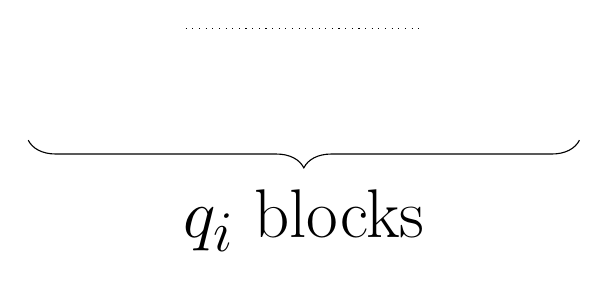
\begin{tikzpicture}
        \startb{0}{0}
        \middleb{3}{0}
        \draw[dotted] (5, 1) -- (8, 1);
        \middleb{8}{0}
        \startb{11}{0}
        \draw [decorate,decoration={brace,amplitude=10pt,mirror},xshift=0pt,yshift=-12pt]
        (3, 0) -- (10, 0) node [below,black,midway,yshift=-0.5cm]
        {\Huge $q_i$ blocks};
    \end{tikzpicture}
    }
    \caption{Transformation of \textit{Subset sum} element $q_i$}
    \label{fig:wells}
\end{figure}

When placing the first block it is evident that we have only two choices: place the $\mathbf{H}_H$ block column 2-3 of any well. This transform the chosen well from a closed to an open state. We then proceed to placing the middle $q_i$ blocks. When deciding the outcome of these placements the following lemmas are of use:\\

\begin{lem}
TODO: prove that the height doesn't change in the columns in phase 1. Important for second lemma.
\end{lem}

\bigbreak

\begin{lem}
In phase 1, placing a $\mathbf{H}$ block in any other column than 4-5 in a well will make the same well permanently closed.
\end{lem}

\begin{proof}
In the first case, the well is closed. We can only place the $\mathbf{H}$ block in column 2-3. Since no cells are cleared as a result, column 1 to 4 are filled except for the top two rows. We therefore cannot place any block in these columns without a game over. Either the column right of column 5 is filled, or the gameboard has ended. Since column 4 is also filled, we cannot place any block in column 5. Thus the well is permanently closed.

In the second case, the well is open. Apart from column 4-5, we can only place the $\mathbf{H}$ block in column 3-4. This does not clear any cells as a result. Thus with the same arguments as in the first case, the well is permanently blocked.
\end{proof}
